\documentclass{article}

\usepackage{graphicx}

\author{Nic Hollingum - 308193415}
\title{Computational Geometry - Assignment 4}

\addtolength{\oddsidemargin}{-.875in}
\addtolength{\evensidemargin}{-.875in}
\addtolength{\textwidth}{1.75in}
\addtolength{\topmargin}{-0.5in}
\addtolength{\textheight}{1.5in}

\begin{document}
\maketitle

\section {Euclidian Problems}

\subsection*{a}
By the triangle inequality, this is trivial, we shall prove it by contradiction.
We have a cycle of nodes which we vist, and removing nodes from the cycle represents removing elements to form a subset.
Conversely adding nodes represents increasing a subset to the size of the set.
In order for a subset not to be shorter than the superset, then there must exist some superset shorter than its subset.
In other words we have to decrease the length of the cycle by adding a node, or, we stop at some node in the cycle, move to the new node, then back to the next node in the cycle and continue.
But this requires the sum of paths from some node in the cycle to new node, and new node back to next, be less than some node to the next, which violates the triangle inequality (if a, b and c are edges of a triangle, then the length of any 1 must be less than the sum of the other 2).

\subsection*{b}
Proof by example:

\begin{figure}[htb]
\begin{center}
\leavevmode
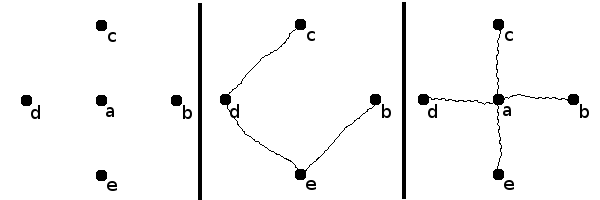
\includegraphics[width=0.6\textwidth]{mst.png}
\end{center}
\end{figure}
\label{fig:mst}

Using the 5 points here, where our subset lacks point $a$, we see that the MST grows longer.
When $a$ is absent, we must choose 3 of the 6 edges in $k_4$, and the 3 shortest edges are those around the perimeter.
Each of the perimeter points is 1 unit up, down, left or right of $a$, and the border edges have length $\sqrt 2$ accordingly, the total length is $3 \sqrt 2 = 4.24$.
When $a$ is present then the MST is 4 edges from $a$ to all of the corner points.
Each corner point is 1 unit distance from $a$, and so the MST has length 4, which is less than above.
Therefore even though the middle graph is a subset of the left, it has a longer MST than the right.

\subsection*{c}
First TSP must be more than MST, this can be verified by a counting problem, and that MST is a tree and TSP is a cycle.
given n points, where each is equidistant from evey other (we need n-1 dimensions to do this by the way) we note that the MST must have n-1 edges and so n-1 length, but the cycle must return to its start node, and so must have n edges and n length.
If the points are not equidistant we know that if the TSP is able to choose a shorter path, the MST is as well, but there are times when the MST can avoid long paths where the TSP cant.
Consider many points spread out evenly along a circle edge, with a gap on one side.
The MST is able to avoid this gap and simply choose the points around the perimeter, wheres at TSP will either take this edge, or backtrack along other edges and so waste time.

We also note that given an MST, we are able to find some repeating cycle, using depth-first search along all branches of the tree.
The salesman starts at some node in the tree and traverses it depth first.
Each edge must be crossed once to go to new nodes, and again later to return prom them, hence exactly twice.
Therefore we have a repeating cycle no more than double the length of the MST which visits every node.
Clearly a more efficient TSP can be contrived by skipping nodes we know we have visited and we will return from.
Such that if we would return from a to b, then b to it's parent c, we simply go from a to c and save the distance, therefore optimal TSP must be less or equal to 2*MST.

\section {Voronoi Convex Hull}

This question can be posed more formally: For which pairs of points can we place an infinitely large circle such that the circle intersects both points and no others.
Clearly such a circle constitutes an unbounded barrier between cells in the Voronoi diagram.
If we can place such a circle then all the points in the triangle between its centre, the radial line joining the centre to one of the points, and a segment meeting the line between both points perpendicular (a right angled triangle) belongs to the cell for that point, and the mirror for the other cell.
Since the circle is infinitely large the area of the triangle can be infinitely large and the region is unbounded.

Furthur there can exist no unbounded cell for which such a circle cannot be constructed.
Consider the unbounded barrier between 2 unbounded cells.
Clearly if a cell is unbounded it must have at least 1 unbounded barrier (though usually 2), and therefore there must be other unbounded cells neighbouring this one.
Where $n=2$ the voronoi diagram is defined but the convex hull is just a line, therefore the result is trivially obvious.
Given we have unbounded barriers we are able to pick a point infinitely far out along the barrier and call this the circle's centre.
Then when we draw the circle no other point in the set will be inside the circle, since this is the definition of barriers in the Voronoi diagram

Now we must show that such circles can only be found (and are always found) between adjacent points in the convex hull.
As the circle's radius increases to infinity the arc between the 2 chosen points approaches a straight line.
Indeed for sufficiently (and we have all of infinity to work with) large circles we can extend this line to infinity and it will converge with the arc.
So we can view the circle as actually defining a half-space to one side of the pair of points.
We had wished to find circles which could be infinitely large and had no points inside them, and only the 2 points on their circumferance.
But now we can say we are looking for pairs of points where no other point exists in the half space to one side of them.
This is precisely the definition of an edge of the convex hull.

\section {MST and Delauny}

\subsection*{a}
{\em We presume this is in euclidian space, for a general graph this statement is untrue, please excuse the verbose descriptions, my diagram authoring skills are not up to scratch}

Consider the angle between these edges in the MST.
We know that these edges all meet at a point $a$ of degree $d$.
Then either all angles are ${2\pi} \over d$ or one is less.
Now we observe that this minimal angle must satisfy a triangular constraint where the edges beteen the 2 points that construct it and $a$ are lesss than the distance between these 2 points.
This is stated formally by basic trigonometry: $a^2 = b^2 + c^2 - 2bc\cos{A}$, in which $b$ and $c$ are the MST edges and $a$ is the distance between the 2 points.
We Then must be able to find a $b$ and $c$ such that both are less than $a$.

In the case where the degree is 6, the minimal angle is $\pi \over 3$ and hence $a^2 = b^2 + c^2 - bc$.
Fixing $b$ of length 1 we can clearly see that $a > c$ when $c <= 1$, however when $c < 1$, $a$ becomes imaginary, so clearly $c$ must be 1 aswell.

However when we must accomodate degree 7 then the minimum angle is ${{2\pi} \over 7} \approx 0.8976$ or less and our cosine rule becomes $a^2 \approx b^2 + c^2 - 1.247 b c$.
If we suppose b and c are equidistant from a (let us call this distance 1) then $a^2 \approx 0.753$ and $a$ is less than $b$ and $c$.
If they were not equidistant Then we are able to draw a circle with center at the more distant, then less distant must somehow be inside the sector with width ${2\pi} \over 7$ and closer than the more distant point.
However this entire sector is contained within the circle with center at the more distant, and so any point inside it is closer to the more distant point than the more distant is to $a$.

Therefor this is a contradiction, and it is impossible to construct those 2 edges of the MST whose angular difference is less than or equal to ${2 \pi} \over 7$.
It is therefore impossible to construct a Euclidian MST with degree greater than 6, since 2 such edges must exist in it.

\subsection*{b}

Our pointset is a single point $a$ in the centre with $n-1$ points arranged evenly around the circumfrence of a circle.
We will show that there is only 1 valid way to delauny triangulate this region, and that the central point will always have degree n-1.

Consider the Voronoi diagram of this pointset.
At the center will be a regular polygon with $n-1$ edges.
The centre of each edge will be equidistant from the central point and one of the points on the circumfrence.
At each vertex of the polygon a half-line will be cast outwards between 2 points on the circumfrence.
The important consideration is that this central polygon borders the unbounded cell of every point on the circumfrence, which there are $n-1$ of.
Therefore in the delauny triangulation, the central point will have $n-1$ delauny edges joining it.

\section {Interval Range Query}

This problem can be solved using a 2D Range tree with fractional cascading.
In lectures it was observed that 2d range trees use $O(n \log n)$ space, $O(n \log n)$ preprocessing, and with fractional cascading we can solve in $O(\log n + k)$ time.
We shall co-opt the method described in lectures for solving 2D range queries with fractional cascading by converting our problem into a 2D problem, and our queries into 2D queries.

Our dataset are 1D intervals with a start and end point, and our queries are for all intervals with a startpoint greater than $x$ and an endpoint less than $x'$.
This converts to 2 1D queries (and hence 1 2D query) nicely, we want all intervals with a startpoint between $x$ and $\infty$, then all endpoints between $-\infty$ and $x'$.
If we draw our ``intervals'' as 2D points then let us choose arbitrarily that the startpoint maps to x and the endpoint to y.
So our query is now looking for points inside the rectangle undbounded to the right and below.
Only points which start before $x$ will be to the left of the right bound of the rectangle, and only those that end before $x'$ will be below the upper bound.

Now this problem can be solved just like a normal 2D Range query.
Simply return all ``points'' that lie inside the unbounded rectangle.
This requires $O(\log n + k)$ time so long as we use fractional cascading.
The actual procedure for constructing and querying these trees is discussed in lectures, it will not be reiterated here.

\section {t-Spanner}

{\em The proof for part a is lacking, but part a is required to do b, which is easy if we can assume a, so we shall.  Some attempt has been made to show the truth of a's claim, differentiation is involved.}

\subsection*{Lemma 1}
First we examine the bounds on $\tau$.
When it approaches $\pi \over 4$, T approaches infinity, at which point it is sufficient to say that $|uv| \geq |vw|$ by the triangle inequality, and therefore the proposition holds.
Similarly when it approaches 0, T may be as low as 1, at which point again the simple argument that $|uv|$ is longer means the proposition holds.

We can calculate $|vw| \leq \sqrt{|uv|^2 + |uw|^2 + |uv||uw| \cos \tau}$ to gain some insight into the problem.
We are trying to find instances where $t$ can be small enough that $t|vw| + |uw| > t|uv|$ in order to disprove by contradiction, if such instances cannot exist then this suffices as proof for the lemma.
We see easily that $|uv| > |vw|$ since if this were not true, w must either be outside the sector or furthur from u than v.
Given this making t large is not an option for disproving the lemma, since $|uv|$ will always grow faster.
Looking at the function we note that the LHS monotonically increases as w approaches u for sufficiently large t.
This is demonstrated by the above application of the cosine rule, versus the corollary that when w and u share a point, $|vw| = |uv|$.
If we fix $\tau$ and $|uv| = 1$ this also fixes the minimal value of t, and the LHS is maximised when $|uw| + t|vw|$ is maximised, or when $|uw| + t\sqrt{|uw|^2 + 1 + |uw| \cos \tau}$ is maximised.
Given $t \geq {1 \over {\cos \tau \sin \tau}}$ the minimal value of t can also be presumed, hence $|uw| + {\sqrt{|uw|^2 + 1 + |uw| \cos \tau} \over {\cos \tau \sin \tau}}$.

This gives us our intuition that the choice of $\tau$ affects the maximal choice of LHS and hence whether the lemma holds.
Then it is sufficient to say that as $\tau$ increases linearly, $|vw|$ increases sublinearly for any choice of $\tau$, which means that if The lemma holds for the extreme values shown above, it must hold for values in between.
Therefore there exists no value of $\tau$ for which $|uw| + t|vw| > t|uv|$ and hence the lemma holds.

\subsection*{Spanner induction}

Let us add an edge from every poing the the graph to the $k$ nearest points inside $k$ sectors surrounding the point.
In the base case we have 2 points with an edge between them whose edge equals the euclidian distance, and hence this is a t-spanner.

When we add a new point we shall add up to k edges from it to existing nodes in the graph.
Clearly the graph is connected, since all new vertices must add at least 1 edge in the case when the entirety of the current graph is in 1 of the k sectors.
Therefore there is a path from every vertex to every other vertex.
When we added a new point it connected to the current graph by some arc, at which point paths to new vertices could flow through that arc.
From the base case we saw that all paths had distance equal to euclidian distance, however now we shall show that after n additions, all paths have distance at most t times the euclidian distance.
From lemma 1 we saw that in any sector, t times the distance between the new point and some far point was greater than the distance between the new point and the closest plus t times the distance between this closest point and the far one.
This can be recursively applied by choosing the closest point as the ``new point'' and looking in the sector which contains the furthur point.
We substitute the inequality from this second hop into the first for points $a, b, c, d$: the new point, its closest point, the closest point to b in b's sector containing d, and the farthest point respectively, to get $|ab| + |bc| + t|cd| \leq |ab| + t|bd| \leq t|ad|$.
Simply continuing in this fashion, eventually we will reach a point where d is the closest in the sector containing d, and we wll not have ever exceeded t times the distance $ad$.

Hence the graph constructed by the above description is a t-spanner.

\subsection*{Linearity}
The number of edges in the graph is linear in the number of points.
This is a trivial observation that for a given t, $\tau$ is chosen maximally for efficiency and hence $k$ is minimal and fixed.
Therefore since we draw an edge between each node n and the nearest neighbour inside each of the k sectors, there are at most $nk$ edges.
Since k is constant this means $O(n)$ edges.

\end{document}
